\centerline{\Huge \bf  Тренировочная Олимпиада 1}
\centerline{\Huge \bf 7 класс}
\centerline{\Huge \bf Уровень: городская Олимпиада.}


\begin{flushright}
    \scriptsize{Глава 1. Начало конца.}
\end{flushright}


\problem{1} 
Татары считают, что среднее количество поедаемого чак-чака их населением в 41 раз превосходит среднее количество поедаемого чак-чака всеми жителями России (включая всех татар). Докажите, что татары лукавят. Население татарстана составляет 2,5\% от населения России.
\begin{flushright}
    \textit{\small{(Гасанов Р.В.)}}
\end{flushright}

\problem{2}
Расул Владимирович и Анджур Аркадьевич принесли две коробки БэйбиФоксов в первой коробке лежало 12355780891 конфета, а во второй коробке лежало 37289134097 конфет. И сказали они разделить конфеты на Шиншилл Лососей и Киви поровну. Но Дольган не поверил им наслово, что такое количество конфет можно поделить на 3. Дольган что-то знает, а что-то не знает. Поэтому долго не мог понять можно ли все-таки их разделить. Пока рядом не прошел Герман и в шутку переложил несколько конфет из второй коробки в первую. И тогда Дольгану стало всё очевидно. Какое наименьшее количество конфет Герман переложил?
\begin{flushright}
    \textit{\small{(Очиров О.В.)}}
\end{flushright}

\problem{3}
Очиру Владимировичу было лень придумывать задачу на олимпиаду. И он взял рандомную олимпиаду из интернета, в которой было 23 слова и все они были различными, добавил по две копии всех слов и перемешал в случайном порядке. Сколько различных задач он мог составить?

\textit{Примечание:} Задачи Очира Владимировича настолько гениальны, что любый набор слов можете считать задачей.
\begin{flushright}
    \textit{\small{(Очиров О.В.)}}
\end{flushright}

\begin{wrapfigure}{r}{0.35\linewidth}
    \centering
    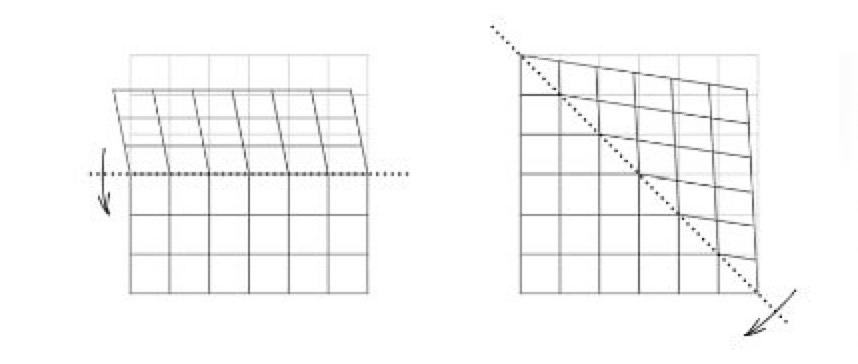
\includegraphics[width=\linewidth]{VII блок/Киви/lesson_6/Picture_7.1.4_1.jpg}
\end{wrapfigure}

\problem{4}
Эльзята на уроке в художке закрасила на клетчатой бумаге размера $6\times 6$ несколько клеток и отдала листочек Эвене. Та согнула листочек пополам сначала по горизонтали, потом по диагонали так как показано на рисунке. Если закрашенная клетка соприкасалась с незакрашенной, то незакрашенная покрасится. Сколькими способоами Эльзята могла закрасить пустой листок бумаги $6 \times 6$ так, чтобы после действий Эвены получилась фигура с рисунка.
\begin{flushright}
    \textit{\small{(Гасанов Р.В.)}}
\end{flushright}

\begin{figure}[h]
\centering
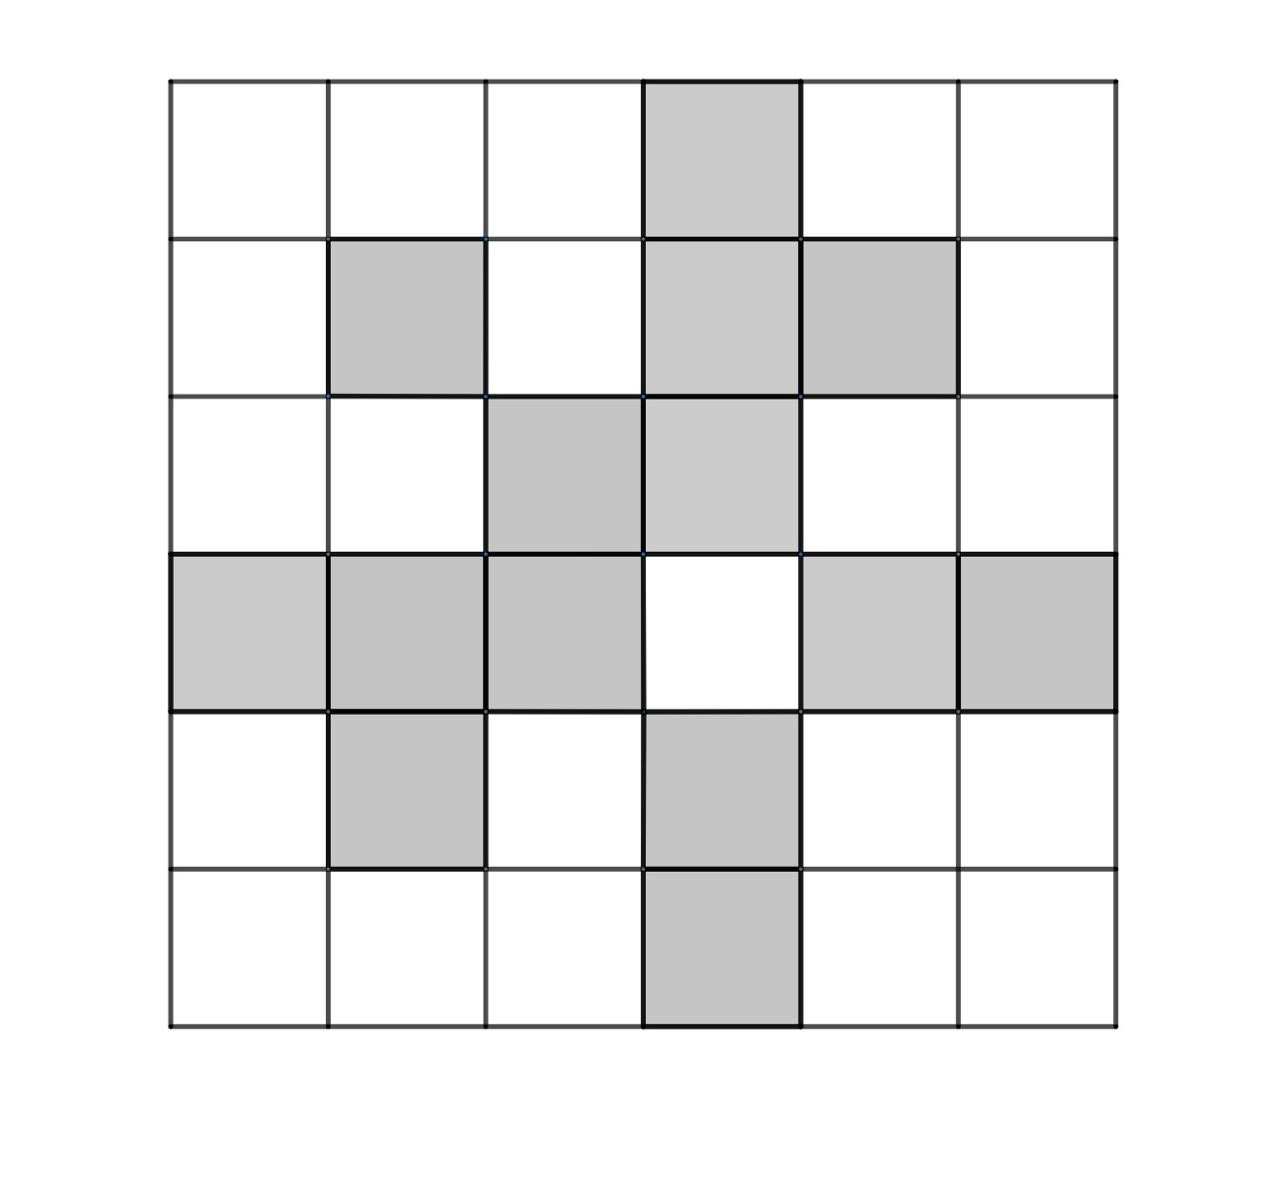
\includegraphics[width=0.25\linewidth]{VII блок/Киви/lesson_6/Picture_7.1.4_2.jpg}
\end{figure}

\problem{5}
Где закрашенная площадь больше $-$ под диагональню или над диагональню?

\begin{figure}[h]
\centering
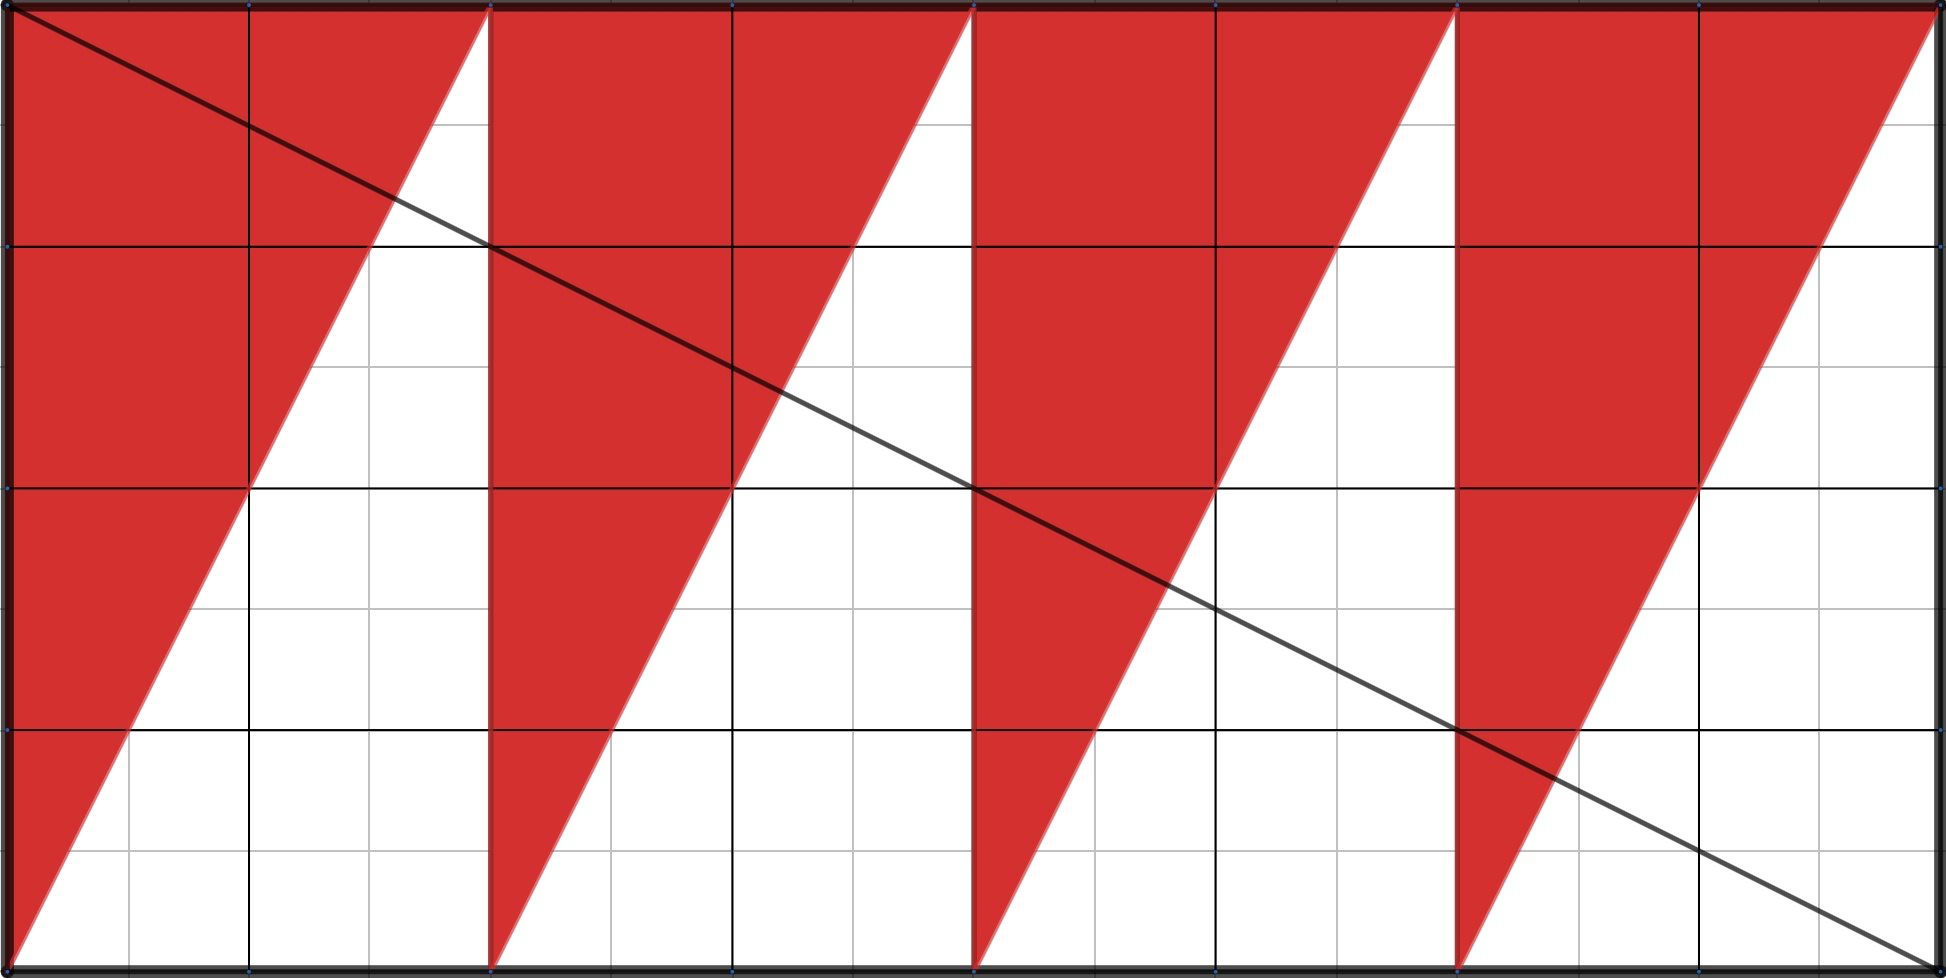
\includegraphics[width=0.5\linewidth]{VII блок/Киви/lesson_6/Picture_7.1.5.png}
\end{figure}